\chapter{Self-consistent field approximation} \label{ch:3}

\section{The many-electron problem}
Suppose we have an Fe atom. It consists of a positively charged heavy nucleus
and 26 negatively charged electrons. Unlike the one-electron systems we had before,
each of those 26 electrons will not only feel the attraction from the nucleus,
but will also experience the repulsions from all the other electrons. The interactions
among electrons are rather complicated. But the real challenge comes from how
one should represent the many-body wave function numerically. For 26 electrons,
we have the wave function $\Psi(\vec{r}_1,\vec{r}_2,\ldots,\vec{r}_{26})$, or
in Cartesian coordinates $\Psi(x_1,y_1,z_1,x_2,y_2,z_2,\ldots,x_{26},y_{26},z_{26})$.
This wave function has a dimension $3 \times 26 = 78$. To get an impression how
crazy this dimension is, let's take a ``toy'' grid with 10 grid points per
dimension. Then the total number of points on our toy grid will be $10^{78}$.
What does it imply? If the wave function on each point is a double precision
floating point number, it would require us $64 \times 10^{78}$ bits to store the wave function
on just this toy grid. Not impressive enough? Let's say if one bit could be stored on
just one atom, $64 \times 10^{78}$ atoms is already beyond the amount of substances
in the observable universe! So are you still thinking about storing it on your small
laptop?

Nobody was able to store such a wave function on a hard disk. But that is not
the end of our story. An important step to get rid of this huge dimension
is to make an ansatz: the many-body solution can be written as products of
one-particle wave functions
\begin{equation} \label{eq:oneProds}
\Psi(\vec{r}_1,\vec{r}_2,\ldots,\vec{r}_N) \approx \varphi_1(\vec{r}_1)\varphi_2(\vec{r}_2)\ldots\varphi_N(\vec{r}_N)
\end{equation}
It is important to notice that Eqn.~(\ref{eq:oneProds}) is really an approximation.
It assumes that electrons are distinguishable which is, however, not true.
The famous Pauli exclusion principle is not included here as the wave function
given by Eqn.~(\ref{eq:oneProds}) is not anti-symmetric.\footnote{An alternative
ansatz that includes the anti-symmetric property of electron wave functions
is the Slater determinant formulation, which leads to the Hartree-Fock method
of solving many-electron problems. Our methods here are based on the density
functional theory which starts from the Kohn-Sham equation and
Eqn.~(\ref{eq:oneProds}) will be the right ansatz for us to use.}
Therefore, we must take extra care for the electron configurations, i.e.\
how one puts electrons onto different orbitals. But with Eqn.~(\ref{eq:oneProds}),
a ``$3N$ dimensional'' wave function is decomposed into $N$ ``3 dimensional''
wave functions. This is really a great milestone. We are
not anymore embarrassed by the non-handleable gigantic wave functions. Instead,
we have $N$ lovely 3-dimensional one-electron wave functions. But that is not
good enough. Because those $N$ electrons are coupled to each other. In order to handle
those $N$ wave functions separately, one must think about a way to decouple them.
Recall our Schr\"{o}dinger equation, for general $N$, Eqn.~(\ref{eq:Schr}) (in a.u.) reads
\begin{equation} \label{eq:SchrMany}
\left\{\sum_{i=1}^N \left[ -\frac{1}{2} \nabla_i^2 - \frac{Z}{r_i} \right] + \sum_{i<j}^N \frac{1}{|\vec{r}_i - \vec{r}_j|}\right\} \Psi = E \Psi
\end{equation}
By analyzing this equation, we easily find out that the second term in the curly
brace is causing the trouble that all electrons are coupled together.
If one could decouple this electron-electron interaction, the problem will
become as easy as for the one-electron case. That is where the self-consistent
field approximation plays an important role. It suggests us to approximate the
electron-electron repulsion term by a spherically symmetric mean-field potential
\begin{equation} \label{eq:Hartree}
\sum_{i<j}^N \frac{1}{|\vec{r}_i - \vec{r}_j|} \approx  V_{\text{Hartree}}(r)
\end{equation}
%
This $V_{\text{Hartree}}(r)$ is called the Hartree potential. Under this mean-field
approximation, the $N$ electrons are not coupled anymore. The equation
\begin{equation} \label{eq:SchrDecp}
\left\{\sum_{i=1}^N \left[ -\frac{1}{2} \nabla_i^2 - \frac{Z}{r_i} \right] + V_{\text{Hartree}}(r)\right\} \Psi = E \Psi
\end{equation}
can be decomposed into
\begin{equation} \label{eq:SchrOnes}
\left[ -\frac{1}{2} \nabla^2 + V_{\text{ext}}(r) +  V_{\text{Hartree}}(r) \right] \varphi_i = E_i \varphi_i \quad \text{for } i = 1,2,\cdots,N
\end{equation}
where $V_{\text{ext}}(r) = -Z/r$ is the external potential from the nucleus.
In fact, a so called exchange-correlation potential $V_{\text{xc}}(r)$ should
be added into the Hamiltonian to include the exchange-correction effect \cite{ES}
from the electrons:
\begin{equation} \label{eq:SchrOnesXC}
\left[ -\frac{1}{2} \nabla^2 + V_{\text{ext}}(r) +  V_{\text{Hartree}}(r) + V_{\text{xc}}(r) \right] \varphi_i = E_i \varphi_i \quad \text{for } i = 1,2,\cdots,N
\end{equation}
%
This is the Kohn-Sham equation \cite{KS} that we are going to solve.
If we compare Eqn.~(\ref{eq:SchrOnesXC}) with Eqn.~(\ref{eq:SchrOne}), we
immediately see that they are exactly the same except the potential here has
three terms. This is how we break down a
non-solvable many-electron problem into solvable one-electron problems.
If you still remember how we solved the one-electron case in the previous chapter,
we used a separation of variable technique to separate the 3-dimensional ODE
into a radial equation and an angular equation. While the solutions for the angular
equation are known already, our task is to solve the radial equation:
\begin{equation} \label{eq:manyElec}
\boxed{-\frac{1}{2} \frac{d^2u_i}{dr^2} + \left[ V_{\text{ext}}(r) +  V_{\text{Hartree}}(r) + V_{\text{xc}}(r) + \frac{l(l+1)}{2r^2} \right] u_i = E_i u_i} \quad \text{for } i = 1,2,\cdots,N
\end{equation}
with the same boundary conditions: $u(r) \propto r^{l+1}$ as $r\rightarrow0$ and
$u(r) \propto \exp{(-\sqrt{-2E}r)}$ as $r\rightarrow\infty$.

Again, Eqn.~(\ref{eq:manyElec}) is identical to Eqn.~(\ref{eq:oneElec}) except
the potential for the many-electron case is more complicated. While $V_{\text{ext}}(r)$
is given already, the two other potentials $V_{\text{Hartree}}(r)$ and $V_{\text{xc}}(r)$
remain unknown to us. But suppose we knew the exact expression for those
two potentials, we would be able to solve Eqn.~(\ref{eq:manyElec}) as
easily as we did in the previous chapter. Unfortunately, we do not have them
explicitly. So one might complain: how are we supposed to solve a differential
equation without knowing the differential equation? This is quite a reasonable
question and the answer is: No, we cannot solve it within one step like what we did for
the one-electron case. But with a self-consistent iterative scheme we would be able to
achieve the solution. The idea is the following:

Since we do not know $V_{\text{Hartree}}(r)$ and $V_{\text{xc}}(r)$, we guess.
We start from an initial guess of the two unknown potentials,
say, $V_{\text{Hartree}}^0(r)=0$ and $V_{\text{xc}}^0(r)=0$.\footnote{Zero
Hartree and zero exchange-correlation potentials imply the
electrons are not interacting, which will result in the same solutions as for the
one-electron problems.}
From this initial guess, we obtain a solution $\{u_i^0(r)\}$.\footnote{Here
the notation $\{u_i(r)\}$ denotes the complete set of
$u_i(r)$ for $i=1,2,\ldots,N$. With a superscript $k$, $\{u_i^k(r)\}$ indicates
the solution at the $k$-th iteration.}
Next, we use this solution to update $V_{\text{Hartree}}^1(r)$ and $V_{\text{xc}}^1(r)$
and obtain a new solution $\{u_i^1(r)\}$. This loop continues until $V_{\text{Hartree}}^k(r)$
and $V_{\text{xc}}^k(r)$ (and consequently the solution $\{u_i^k(r)\}$) converge.
Fig.~\ref{fig:scfFlow} illustrates the iteration scheme of the self-consistent field
computation. The loop starts from an initial potential and continues updating the
potential until the solution converges. That is why we call this scheme the self-consistent
method: the wave functions produce the potential and the potential produces wave functions,
which is self-consistent.

\begin{figure}[h!]
\centering
\footnotesize
\tikzstyle{cloud}    = [ellipse, draw, text width=4.0em, text badly centered, minimum height=2em]
\tikzstyle{block}    = [rectangle, draw, rounded corners, text width=4.5em, text badly centered, minimum height=4em]
\tikzstyle{decision} = [diamond, draw, text width=4.5em, text badly centered, aspect=1.5]
\tikzstyle{line}     = [draw, -triangle 45]
\begin{tikzpicture}[node distance = 9em, auto]
% Place nodes
\node [cloud] (init) {initial potential};
\node [block, right of=init] (orbital) {compute $\{u_i(r)\}$};
\node [block, right of=orbital] (potential) {compute $V_{\text{Hartree}}(r)$ $V_{\text{xc}}(r)$};
\node [block, below of=potential, node distance=5em] (update) {update $V_{\text{Hartree}}(r)$ $V_{\text{xc}}(r)$};
\node [decision, right of=potential] (converge) {converged?};
\node [cloud, right of=converge, text width=2.5em,] (stop) {stop};
% Draw edges
\path [line] (init) -- (orbital);
\path [line] (orbital) -- (potential);
\path [line] (potential) -- (converge);
\path [line] (converge) |- node [near start] {no} (update);
\path [line] (update) -| (orbital);
\path [line] (converge) -- node {yes}(stop);
\end{tikzpicture}
\caption{Flow chart of self-consistent field iteration. The loop starts from an
initial potential and continues updating the potential until the solution converges.}
\label{fig:scfFlow}
\end{figure}

Most of the steps in Fig.~\ref{fig:scfFlow} are clear to us. For example, the
computation from a given potential to the wave functions has been discussed
thoroughly in the previous chapter. What we need to do is simply replacing $V(r)$
in Eqn.~(\ref{eq:oneElec}) by $V_{\text{ext}}(r) +  V_{\text{Hartree}}(r) + V_{\text{xc}}(r)$.
The convergence test in the ``diamond'' could be checked by comparing the old total energy
with the new total energy of the system.\footnote{Computation of the total energy
will be discussed in the later section.} What still remains unclear to
us is the step from a set of given wave functions to obtaining the new potentials
$V_{\text{Hartree}}(r)$ and $V_{\text{xc}}(r)$.

\section{The Hartree potential}
The computation of the Hartree potential requires not too much knowledge
from quantum mechanics but almost purely electrostatics as you might
have learned in your school. The keywords are: charge density, charge,
electric field and electric potential. As a brief review, the relations
among those quantities are summarized below.

Imagine we have a charged object with charge density $\rho(\vec{r})$,
the total charge enclosed in volume $\mathcal{V}$ is the volume integration
over the charge density
\begin{equation} \label{eq:charge}
Q_{\text{enc}} = \int_{\mathcal{V}} d^3r\,{\rho(\vec{r})}
\end{equation}
For a spherical symmetrically distributed charge density $\rho(r)$, the total
charge enclosed in a sphere with radius $r$ can be integrated using
spherical coordinate system
\begin{equation} \label{eq:charger}
Q(r) = \int_0^{2\pi}d\phi \int_0^{\pi}d\theta\,\sin{\theta} \int_0^r dr'\,r'^2\,\rho(r') = 4\pi \int_0^r dr'\,r'^2\,\rho(r')
\end{equation}
The electric field created by the enclosed charge can be computed easily
(recall Coulomb's law)
\begin{equation} \label{eq:eleField}
\vec{E}(r) = \frac{1}{4\pi\varepsilon_0} \frac{Q(r)}{r^2} \hat{\vec{r}} \stackrel{\text{in a.u.}}{=\joinrel=} \frac{Q(r)}{r^2} \hat{\vec{r}}
\end{equation}
Meanwhile, the electric field is the negative gradient of the electric potential
$\vec{E}(r) = -\boldsymbol{\nabla} V(r)$ and $V(r\rightarrow\infty)\equiv0$. Hence,
\begin{equation} \label{eq:elePot}
V(r) = - \int_{\infty}^{r} dr'\, \vec{E}(r') \cdot \hat{\vec{r}} = \int_{r}^{\infty}dr'\, E(r')
\end{equation}

Now let's do a small exercise:

\paragraph{Question:}
Suppose we have a uniformly charged sphere (Fig.~\ref{fig:sphere})
of radius $R$ with charge density $\rho(r) = \frac{3}{4\pi R^3}$.
What is the electric potential it creates?
\begin{figure}[h!]
\centering
  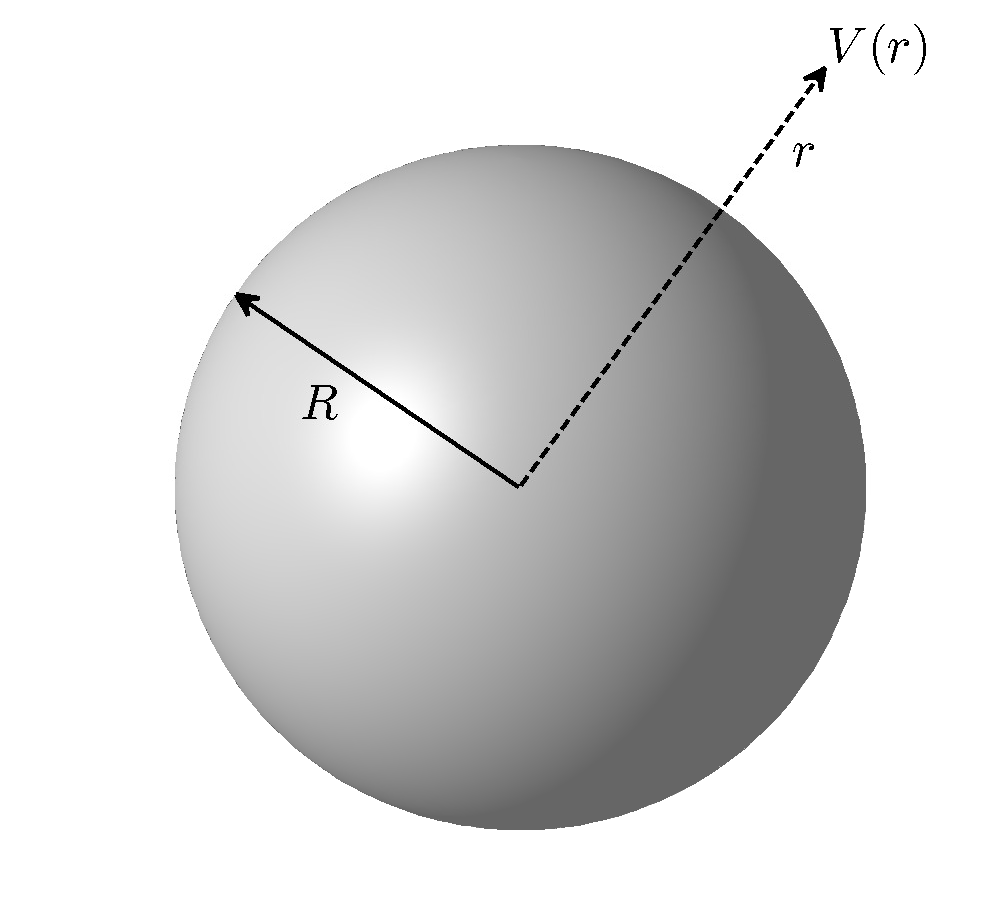
\includegraphics[width=0.4\textwidth]{sphere}
  \caption{A uniformly charged sphere of radius $R$ with charge density $\rho(r) = \frac{3}{4\pi R^3}$.}
  \label{fig:sphere}
\end{figure}

\vspace{5em}
\paragraph{Solution:}
Since there is a discontinuity on the sphere's surface, we'd better solve
the problem casewise.

For $r > R$,
\begin{align} \label{eq:uniCharge>}
Q(r) & = 4\pi \int_0^R dr'\,r'^2\, \rho(r') = 1 \\
E(r) & = \frac{Q(r)}{r^2} = \frac{1}{r^2} \\
V(r) & = \int_{r}^{\infty} dr'\, E(r') = \frac{1}{r}
\end{align}
%
For $r \le R$,
\begin{align} \label{eq:uniCharge<}
Q(r) & = 4\pi \int_0^r dr'\,r'^2\, \rho(r') = \frac{r^3}{R^3} \\
E(r) & = \frac{Q(r)}{r^2} = \frac{r}{R^3} \\
V(r) & = \int_r^\infty dr'\, E(r')
       = \int_r^R dr'\, \frac{r'}{R^3} + \int_R^\infty dr'\, \frac{1}{r'^2}
       = \frac{1}{2R} - \frac{r^2}{2R^3} + \frac{1}{R} \label{eq:uniPot}
\end{align}
%
This is basically the recipe how one calculates the electric potentials.
Of course, electron wave functions are not uniformly charged spheres.
They usually spread out to infinity and have nodes in between. But how
should a normalized wave function ``look like'' analogous to a uniformly
charged sphere? The radial wave function should have the following piecewise constant definition
(sorry for the confusion between the wave function $R(r)$ and the radius $R$):
\begin{equation} \label{eq:uniWF}
  R(r) =
  \begin{cases}
  \sqrt{\displaystyle\frac{3}{R^3}} & \text{if } r \le R \\
  0 & \text{if } r > R
  \end{cases}
\end{equation}
%
Notice that the radial wave function $R(r)$ is normalized
\begin{equation} \label{eq:normR}
\int_0^{\infty} dr'\,r'^2\, |R(r')|^2 = \int_0^R dr'\,r'^2\, \frac{3}{R^3} + \int_R^{\infty} dr'\,r'^2\, 0 = 1
\end{equation}
%
Meanwhile, the angular wave function $Y(\theta,\phi)$ is always normalized
\begin{equation} \label{eq:normY}
\int_0^{2\pi} d\phi \int_0^{\pi} d\theta\,\sin{\theta}\, |Y(\theta,\phi)|^2 = 1
\end{equation}
%
But if we assume the electron wave function is spherical symmetrically distributed,
meaning $Y(\theta,\phi) = \text{a constant} = \sqrt{\frac{1}{4\pi}}$, we get the
relation between the charge density and the radial wave function:\footnote{But wait,
shouldn't the charge density of an electron be negative? Yes, that is true. But as
we are always working with electrons, we use a convention that charge units are negative.
The same idea applies to the electric potential in the Schr\"{o}dinger equation,
which is the electric potential energy per negative charge.}
\begin{equation} \label{eq:chargeR}
\rho(r) = |R(r)Y(\theta,\phi)|^2 = \frac{1}{4\pi}|R(r)|^2
\end{equation}
%
If we have $N$ electrons, the charge density (or electron density) is given by
\begin{equation} \label{eq:eleDens}
\rho(r) = \sum_{i=1}^N|\varphi_i(r,\theta,\phi)|^2 = \frac{1}{4\pi} \sum_{i=1}^N|R_i(r)|^2
\end{equation}
%
Our Hartree potential (finally we come back to our main issue!) is simply the
electric potential generated by this electron density, for which we have already
shown the routine of calculation. Suppose we have our radial wave functions on
a grid, a direct relation between $V_{\text{Hartree}}(r)$ and $\{R_i(r)\}$ is
the following:
\begin{equation}
\boxed{
\begin{aligned}
\rho(r)               & =  \frac{1}{4\pi} \sum_{i=1}^N|R_i(r)|^2 \\
Q(r)                  & = 4\pi \int_{r_{\text{min}}}^r dr'\,r'^2 \, \rho(r') \label{eq:HartreePot} \\
V_{\text{Hartree}}(r) & = \int_r^{r_{\text{max}}} dr'\, \frac{Q(r')}{r'^2} + \frac{N}{r_{\text{max}}}
\end{aligned}
}
\end{equation}
%
The integrals in Eqn.~(\ref{eq:HartreePot}) can be evaluated numerically
from the Simpson's rule as we discussed before. But as you might have noticed already,
there is a slight difference in the integrations here. While normally an
integral $\int_a^b dr\, f(r)$ returns us a ``number'', the integral
$\int_a^r dr'\, f(r')$ returns us an ``array''. But that is not difficult at all.
What we need to do is simply to store each intermediate integrated value
while doing the \texttt{for} loop.
Now, if we take the radial wave function in Eqn.~(\ref{eq:uniWF}) to compute the Hartree
potential according to Eqn.~(\ref{eq:HartreePot}), the numerical solution
should agree with the analytical solution in Eqn.~(\ref{eq:uniPot}) in our exercise.
Fig.~\ref{fig:VH} shows the solution we obtained from numerical integration versus the
analytical solution. And yes, the numerical and analytical solutions happily agree with each other.

\begin{figure}[h!]
\centering
  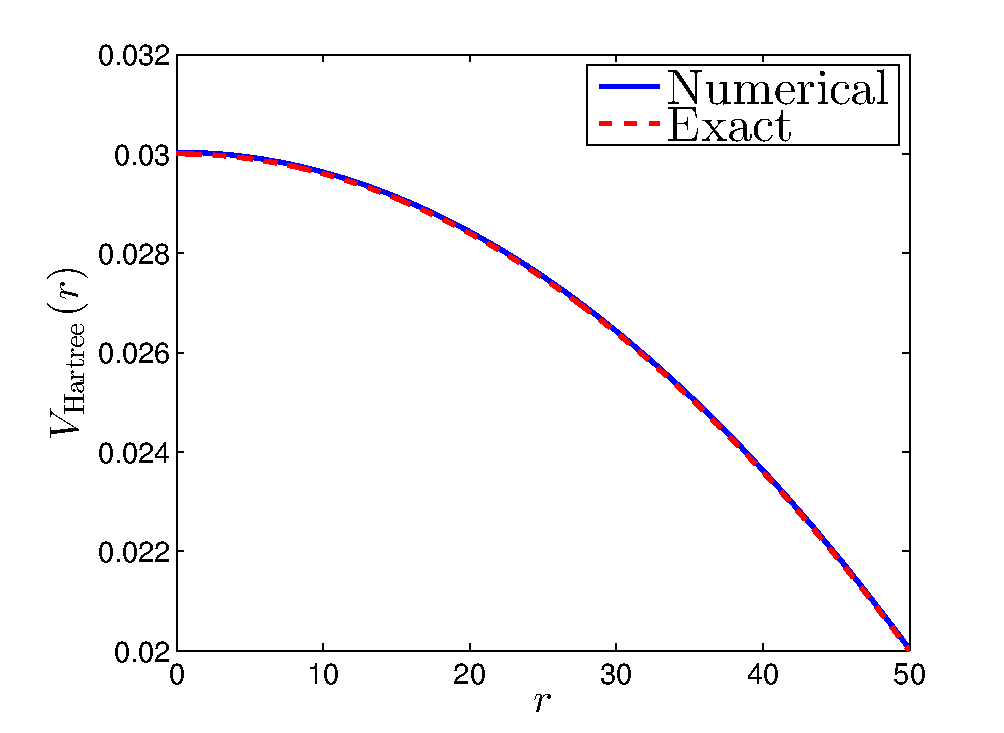
\includegraphics[width=0.5\textwidth]{VH}
  \caption{Numerical (Simpson's rule) and analytical Hartree potentials
           from a normalized wave function
           analogous to a uniformly charged sphere of radius $R=50$.}
  \label{fig:VH}
\end{figure}

\section{The exchange-correlation potential}
The exchange-correlation potential is only a subtle correction\footnote{The
exchange-correlation potential is roughly one order smaller than
the Hartree potential.} but definitely a key for obtaining
accurate self-consistent solutions. The issue of the exchange-correlation
effects comes from the framework of Kohn-Sham density functional theory (DFT) \cite{KS}, which
exactly maps the many-electron problem onto equivalent one-electron problems. In practical
calculations, the local density approximation (LDA) is usually used to simplify the computation
for the exchange-correlation potentials. LDA makes an assumption that the electron density
$\rho(\vec{r})$ is slowly varying. As a result, the exchange-correlation energy
$E_{\text{xc}}$ can be expressed in terms of the exchange-correlation energy
density $\epsilon_{\text{xc}}$,\footnote{The exchange-correlation energy density $\epsilon_{\text{xc}}(\rho)$
is the exchange and correlation energy per electron of a uniform electron
gas of density $\rho$. If there were no local density approximation, we would not
be able to compute the exchange-correlation energy from a uniform electron gas.} as
\begin{equation} \label{eq:Exc}
E_{\text{xc}}[\rho(\vec{r})] = \int d^3r\, \rho(\vec{r}) \epsilon_{\text{xc}}(\rho(\vec{r}))
\end{equation}
%
The corresponding exchange-correlation potential is given by
\begin{equation} \label{eq:Vxc}
V_{\text{xc}}[\rho(\vec{r})] = \frac{\delta \left( \rho(\vec{r}) \epsilon_{\text{xc}}(\rho(\vec{r})) \right)}{\delta \rho(\vec{r})}
\end{equation}
%
Don't be scared of those functional formulations. What we will do in the end is
simply to input a spherically symmetric electron density $\rho(r)$ and output
the exchange-correlation potential $V_{\text{xc}}(r)$ (Fig.~\ref{fig:LDA}).
There are a number of density functionals to approximate
$V_{\text{xc}}(r)$ from $\rho(r)$. A detailed discussion can be found in Reference
\cite{LDA}. Here we provide the Ceperley-Alder approximation with Vosko-Wilk-Nusair
parameterisation (CA-VWN) which is the density functional recommended by Reference \cite{LDA}.

\begin{figure}[h!]
\centering
\footnotesize
\usetikzlibrary{shapes,arrows}
\tikzstyle{cloud} = [ellipse, draw, text width=3em, text badly centered, minimum height=3em]
\tikzstyle{block} = [rectangle, draw, rounded corners, text width=6.5em, text badly centered, minimum height=4em]
\tikzstyle{line}  = [draw, -triangle 45]
\begin{tikzpicture}[node distance = 9em, auto]
% Place nodes
\node [cloud] (rho) {$\rho(r)$};
\node [block, right of=rho] (LDA) {Local density approximation};
\node [cloud, right of=LDA] (Vxc) {$V_{\text{xc}}(r)$};
% Draw edges
\path [line] (rho) -- (LDA);
\path [line] (LDA) -- (Vxc);
\end{tikzpicture}
\caption{Input a spherically symmetric electron density $\rho(r)$ and output
the exchange-correlation potential $V_{\text{xc}}(r)$.}
\label{fig:LDA}
\end{figure}

First of all, we introduce two notations
\begin{equation} \label{eq:rs}
r_s(r) = \left(\frac{3}{4\pi\rho(r)}\right)^{\frac{1}{3}}
\end{equation}
\begin{equation} \label{eq:alpha}
\alpha = \left(\frac{4}{9\pi}\right)^{\frac{1}{3}}
\end{equation}
%
As the name implies, the exchange-correlation potential consists of two terms
\begin{equation} \label{eq:VxVc}
V_{\text{xc}}(r) = V_{\text{x}}(r) + V_{\text{c}}(r)
\end{equation}
%
The exchange term $V_{\text{x}}(r)$ can be computed from the Kohn-Sham-Gasp\'{a}r
approximation:
\begin{equation} \label{eq:exchange}
V_x(r_s) = -\frac{1}{\pi\alpha r_s}
\end{equation}
%
The correlation term $V_{\text{c}}(r)$ from CA-VWN approximation is a bit more complicated:
\begin{equation} \label{eq:correlation}
V_c(r_s) = \epsilon_c(r_s) - \frac{A}{3}\frac{1+b_1 r_s^{1/2}}{1+b_1 r_s^{1/2} + b_2 r_s + b_3 r_s^{3/2}}
\end{equation}
where,\footnote{There are parameters for both paramagnetic
and ferromagnetic correlation energies. Here we use only the paramagnetic
parameters since we are ignoring electron spins at this stage.}
\begin{center}
\begin{tabular}{ c | r }
  \hline
  Parameter & Paramagnetic \\ \hline
  $A$     &  0.0310907\phantom{0} \\
  $b$     &  3.72744\phantom{000} \\
  $c$     & 12.9352\phantom{0000} \\
  $x_0$   & $-0.10498\phantom{000}$ \\
  $b_1$   &  9.81379\phantom{000} \\
  $b_2$   &  2.82224\phantom{000} \\
  $b_3$   &  0.736412\phantom{00} \\
  $Q$     &  6.15199\phantom{000} \\
  \hline
\end{tabular}
\end{center}
$$ \epsilon_c(r_s) = A\left[ \ln{\frac{r_s}{X(r_s)}} + \frac{2b}{Q}\tan^{-1}{\frac{Q}{2\sqrt{r_s}+b} - \frac{b x_0}{X(x_0^2)}}\left( \ln{\frac{(\sqrt{r_s}-x_0)^2}{X_i(r_s)} + \frac{2(b+2x_0)}{Q}}\tan^{-1}{\frac{Q}{2\sqrt{r_s}+b}} \right) \right] $$
and $X(r_s)=r_s+b\sqrt{r_s}+c$.

\section{Achieving self-consistency}
The calculations for both the Hartree potential and the exchange-correlation
potential have been discussed in the last two sections. The effective Kohn-Sham potential
\begin{equation} \label{eq:Vks}
V(r) = V_{\text{ext}}(r) + V_{\text{Hartree}}(r) + V_{\text{xc}}(r)
\end{equation}
appears much clearer to us now. Our next task is to perform the self-consistent
iteration as illustrated in Fig.~\ref{fig:scfFlow}. To update the potential
for a next iteration, naively, one would like to assign:\footnote{Notice
that the external potential $V_{\text{ext}}(r)=-Z/r$ is independent of iterations.}
\begin{equation} \label{eq:Vupdt}
V^{k+1}(r) \gets V_{\text{ext}}(r) + V_{\text{Hartree}}^k(r) + V_{\text{xc}}^k(r)
\end{equation}
%
This is probably what most people would expect. However, this assignment normally
leads to no convergence. The solutions will oscillate inside a
certain region. Imagine we put electrons initially too close to each other,
in the first step, due to strong repulsions, the electrons will be pushed
very far away. In the next step, because the electrons are sitting too
far from each other, they won't experience much repulsions and will be attracted
back by the nucleus. That is the picture how the solutions oscillate.
To avoid this oscillation, we use a technique called linear mixing.
We assign
\begin{equation} \label{eq:mix}
V^{k+1}(r) \gets (1-\alpha) V^k(r) + \alpha \left( V_{\text{ext}}(r) + V_{\text{Hartree}}^k(r) + V_{\text{xc}}^k(r) \right)
\end{equation}
where $\alpha$ is a number between 0 and 1. If $\alpha=1$, Eqn.~(\ref{eq:mix}) will
be identical to Eqn.~(\ref{eq:Vupdt}), which results in a non-converged solution.
But if $\alpha=0$, there will be no potential update at all. The assignment
$V^{k+1}(r) \gets V^k(r)$ makes the loop never end. So, a reasonable choice should
be somewhere in between 0 and 1, and an empirical value for $\alpha$
could be around 0.3 to 0.5.

\section{Comparison to NIST calculations}
The National Institute of Standards and Technology (NIST) provides a
reference for electronic structure calculations \cite{NIST}, which includes
exactly what we are calculating. It provides us an excellent reference for
checking our solutions.

Similar to Table~\ref{table:eigE}, we again selected the same elements for comparison,
namely H (Z = 1), C (Z = 6), Fe (Z = 26), Ag (Z = 47) and U (Z = 92). In contrast
to Table~\ref{table:eigE}, this time all atoms are neutral. So we reached our
goal of calculating many-electron systems. We list the orbital eigen-energies from our
results versus the results from NIST in Table~\ref{table:SCFeigE}.
Energies are given in units of Hartree (a.u.).
If you watch carefully, there is a subtle difference between Table~\ref{table:eigE}
and Table~\ref{table:SCFeigE} in the second column: Previously, we didn't have
superscripts over the orbital names. They are the occupation numbers, which
means the number of electrons in each orbital. For example $2p^2$ means there are
2 electrons sitting in orbital $2p$. And a complete orbital information, like for C: $1s^2$
$2s^2$ $2p^2$, is called the electronic configuration, which describes the occupations
of all orbitals. The electronic configuration needs to be specified by ourselves
and it has to obey the Pauli exclusion principal. For example, there cannot be
more than 2 electrons in an $s$ orbital and no more than 6 electrons in a $p$ orbital.

\begin{table}[h!]
\caption{Comparison of eigen-energies of the occupied orbitals between my results and
the results from NIST for the selected atoms. Energies are given in units of Hartree (a.u.).}
\label{table:SCFeigE}
\begin{center}
\begin{tabular}{ c | c | r | r | r | r }
  \hline
  Elem & Orbital & My results & NIST results & Abs Error & Rel Error \\ \hline \hline
  H &  $1s^1$  &  $-0.233471$  &  $-0.233471$  &  0.000000  &  0.000000 \\  \hline
  C &  $1s^2$  &  $-9.947725$  &  $-9.947718$  &  0.000007  &  0.000001 \\ 
    &  $2s^2$  &  $-0.500866$  &  $-0.500866$  &  0.000000  &  0.000000 \\ 
    &  $2p^2$  &  $-0.199186$  &  $-0.199186$  &  0.000000  &  0.000000 \\ \hline
 Fe &  $1s^2$  &  $-254.225334$  &  $-254.225505$  &  0.000171  &  0.000001 \\ 
    &  $2s^2$  &  $-29.564863$  &  $-29.564860$  &  0.000003  &  0.000000 \\ 
    &  $2p^6$  &  $-25.551762$  &  $-25.551766$  &  0.000004  &  0.000000 \\ 
    &  $3s^2$  &  $-3.360622$  &  $-3.360621$  &  0.000001  &  0.000000 \\ 
    &  $3p^6$  &  $-2.187521$  &  $-2.187523$  &  0.000002  &  0.000001 \\
    &  $3d^6$  &  $-0.295047$  &  $-0.295049$  &  0.000002  &  0.000007 \\
    &  $4s^2$  &  $-0.197976$  &  $-0.197978$  &  0.000002  &  0.000010 \\ \hline
 Ag &  $1s^2$  &  $-900.324405$  &  $-900.324578$  &  0.000173  &  0.000000 \\ 
    &  $2s^2$  &  $-129.859749$  &  $-129.859807$  &  0.000058  &  0.000000 \\ 
    &  $2p^6$  &  $-120.913362$  &  $-120.913351$  &  0.000011  &  0.000000 \\ 
    &  $3s^2$  &  $-23.678432$  &  $-23.678437$  &  0.000005  &  0.000000 \\ 
    &  $3p^6$  &  $-20.067624$  &  $-20.067630$  &  0.000006  &  0.000000 \\ 
    &  $3d^{10}$  &  $-13.367801$  &  $-13.367803$  &  0.000002  &  0.000000 \\ 
    &  $4s^2$  &  $-3.223088$  &  $-3.223090$  &  0.000002  &  0.000001 \\ 
    &  $4p^6$  &  $-2.086598$  &  $-2.086602$  &  0.000004  &  0.000002 \\ 
    &  $4d^{10}$  &  $-0.298702$  &  $-0.298706$  &  0.000004  &  0.000013 \\ 
    &  $5s^1$  &  $-0.157404$  &  $-0.157407$  &  0.000003  &  0.000019 \\  \hline
  U &  $1s^2$  &  $-3689.356876$  &  $-3689.355141$  &  0.001735  &  0.000000 \\ 
    &  $2s^2$  &  $-639.778647$  &  $-639.778728$  &  0.000081  &  0.000000 \\ 
    &  $2p^6$  &  $-619.108505$  &  $-619.108550$  &  0.000045  &  0.000000 \\ 
    &  $3s^2$  &  $-161.118060$  &  $-161.118073$  &  0.000013  &  0.000000 \\ 
    &  $3p^6$  &  $-150.978963$  &  $-150.978980$  &  0.000017  &  0.000000 \\ 
    &  $3d^{10}$  &  $-131.977338$  &  $-131.977358$  &  0.000020  &  0.000000 \\ 
    &  $4s^2$  &  $-40.528086$  &  $-40.528084$  &  0.000002  &  0.000000 \\ 
    &  $4p^6$  &  $-35.853321$  &  $-35.853321$  &  0.000000  &  0.000000 \\ 
    &  $4d^{10}$  &  $-27.123209$  &  $-27.123212$  &  0.000003  &  0.000000 \\ 
    &  $4f^{14}$  &  $-15.027458$  &  $-15.027460$  &  0.000002  &  0.000000 \\ 
    &  $5s^2$  &  $-8.824083$  &  $-8.824089$  &  0.000006  &  0.000001 \\ 
    &  $5p^6$  &  $-7.018084$  &  $-7.018092$  &  0.000008  &  0.000001 \\ 
    &  $5d^{10}$  &  $-3.866167$  &  $-3.866175$  &  0.000008  &  0.000002 \\ 
    &  $5f^3$  &  $-0.366535$  &  $-0.366543$  &  0.000008  &  0.000022 \\ 
    &  $6s^2$  &  $-1.325969$  &  $-1.325976$  &  0.000007  &  0.000005 \\ 
    &  $6p^6$  &  $-0.822530$  &  $-0.822538$  &  0.000008  &  0.000010 \\ 
    &  $6d^1$  &  $-0.143184$  &  $-0.143190$  &  0.000006  &  0.000042 \\
    &  $7s^2$  &  $-0.130943$  &  $-0.130948$  &  0.000005  &  0.000038 \\ 
  \hline
\end{tabular}
\end{center}
\end{table}

\newpage
\section{Total energy of the system}
While the Kohn-Sham orbital eigen-energies give us a nice description to the
atomic systems, their physical meanings are less obvious (they are only
the solutions from our ansatz (\ref{eq:oneProds})). Another very important quantity
which has a key physical meaning is the total energy of the system.
Naively, one might expect that the total energy of the system $E_\text{tot}$ is
simply the summation from all eigen-energies of the Kohn-Sham orbitals.
\begin{equation} \label{eq:sumEeig}
E_\text{tot} \mathrel{\ooalign{\hss?\hss\cr=}} \sum_{i=1}^N{\varepsilon_i}
\end{equation}

That was a close guess, however not quite true. The discrepancy comes from
the following inequalities:
\begin{align}
E_\text{Hartree} & \ne \sum_{i=1}^N{\Bra{\varphi_i} V_\text{Hartree} \Ket{\varphi_i}} \label{eq:discp1} \\
E_\text{xc} & \ne \sum_{i=1}^N{\Bra{\varphi_i} V_\text{xc} \Ket{\varphi_i}} \label{eq:discp2}
\end{align}
where $E_\text{Hartree}$ is the energy from electron-electron repulsions
(Hartree energy) and $E_\text{xc}$ is the exchange-correction energy.
They are not simply the expectation values of their corresponding potentials.
To get the exact total energy of the system, one has to be more careful:
\begin{align}
E_\text{kin} & = \sum_{i=1}^N{\Bra{\varphi_i} \frac{1}{2}\nabla^2 \Ket{\varphi_i}} \label{eq:Ekin} \\
E_\text{ext} & = \sum_{i=1}^N{\Bra{\varphi_i} V_\text{ext} \Ket{\varphi_i}} \label{eq:Eext} \\
E_\text{Hartree} & =  \frac{1}{2}\int d^3r\, \rho(\vec{r})V_\text{Hartree}(\vec{r}) \label{eq:EH} \\
E_\text{xc} & =  \int d^3r\, \rho(\vec{r})\epsilon_\text{xc}(\vec{r}) \label{eq:Exc'}
\end{align}
where $E_\text{kin}$ is the kinetic energy of the electrons, $E_\text{ext}$
is the energy from the external potential $V_\text{ext}(r)=-Z/r$, and the
total energy of the system is given by the summation of those 4 energies
\begin{equation} \label{eq:Etot}
E_\text{tot} = E_\text{kin} + E_\text{ext} + E_\text{Hartree} + E_\text{xc}
\end{equation}
Each term in Eqn.~(\ref{eq:Etot}) can be evaluated explicitly. But taking the derivative
in the kinetic energy (Eqn.~(\ref{eq:Ekin})) introduces unnecessary numerical errors. With a small trick we
can get rid of the Laplacian:
\begin{align} \label{eq:Elap}
\sum_{i=1}^N{\varepsilon_i} & = \sum_{i=1}^N{\Bra{\varphi_i} \frac{1}{2}\nabla^2 + V_\text{ext} + V_\text{Hartree} + V_\text{xc} \Ket{\varphi_i}} \\
 & = \sum_{i=1}^N{\Bra{\varphi_i} \frac{1}{2}\nabla^2 \Ket{\varphi_i}} + \sum_{i=1}^N{\Bra{\varphi_i} V_\text{ext} \Ket{\varphi_i}} + \sum_{i=1}^N{\Bra{\varphi_i} V_\text{Hartree} \Ket{\varphi_i}} + \sum_{i=1}^N{\Bra{\varphi_i} V_\text{xc} \Ket{\varphi_i}} \nonumber \\
\sum_{i=1}^N{\Bra{\varphi_i} \frac{1}{2}\nabla^2 \Ket{\varphi_i}} & = \sum_{i=1}^N{\varepsilon_i} - \sum_{i=1}^N{\Bra{\varphi_i} V_\text{ext} \Ket{\varphi_i}} - \sum_{i=1}^N{\Bra{\varphi_i} V_\text{Hartree} \Ket{\varphi_i}} - \sum_{i=1}^N{\Bra{\varphi_i} V_\text{xc} \Ket{\varphi_i}}
\end{align}
%
Hence Eqn.~(\ref{eq:Etot}) becomes
\begin{equation} \label{eq:EtotSimp}
\boxed{E_\text{tot} = \sum_{i=1}^N{\varepsilon_i} - \sum_{i=1}^N{\Bra{\varphi_i} V_\text{Hartree} \Ket{\varphi_i}} - \sum_{i=1}^N{\Bra{\varphi_i} V_\text{xc} \Ket{\varphi_i}} + E_\text{Hartree} + E_\text{xc}}
\end{equation}
This exactly agrees with the discrepancy we have mentioned in Eqns.~(\ref{eq:discp1})
and (\ref{eq:discp2}). We suggest the summation of Kohn-Sham orbital energies as our
total energy, then we subtract the ``wrong'' terms and put back the correct ones.
If we expand Eqn.~(\ref{eq:EtotSimp}) and read carefully, we have to pay extra
attention to the iteration numbers:
\begin{align} \label{eq:EtotIter}
E_\text{tot}^k = {} & \sum_{i=1}^N{\varepsilon_i^k} - \int d^3r\, \rho^k(\vec{r})V_\text{Hartree}^{k-1}(\vec{r}) - \int d^3r\, \rho^k(\vec{r})V_\text{xc}^{k-1}(\vec{r}) \nonumber \\
                    & + \frac{1}{2}\int d^3r\, \rho^k(\vec{r})V_\text{Hartree}^k(\vec{r}) + \int d^3r\, \rho^k(\vec{r})\epsilon_\text{xc}^k(\vec{r})
\end{align}
And this will be our final expression to compute the total energy of the system.
To check the correctness and accuracy of our solutions, we again compare our results
with the results from NIST. The comparison is listed in Table~\ref{table:SCFEtot}.
\begin{table}[h!]
\caption{Comparison of self-consistent total energies between my results and
the results from NIST for the selected atoms. Energies are given in units of Hartree (a.u.).}
\label{table:SCFEtot}
\begin{center}
\begin{tabular}{ c | r | r | r | r }
  \hline
  Elem & My results & NIST results & Abs Error & Rel Error \\ \hline \hline
  H    & $-0.445670$     & $-0.445671$     & 0.000001 & 0.000002 \\ \hline
  C    & $-37.425762$    & $-37.425749$    & 0.000013 & 0.000000 \\ \hline
 Fe    & $-1261.092727$  & $-1261.093056$  & 0.000329 & 0.000000 \\ \hline
 Ag    & $-5195.030828$  & $-5195.031215$  & 0.000387 & 0.000000 \\ \hline
  U    & $-25658.420765$ & $-25658.417889$ & 0.002876 & 0.000000 \\
  \hline  
\end{tabular}
\end{center}
\end{table}
